\chapter{Results}\label{cha:results}
\section{Threshold scan}
For the threshold scan, the threshold was varied from NAN to NAN in steps of NAN for a range of high gains,
starting with gain NAN and ending with the maxmial gain of 62.
\newline
The number of hits was measured for each of the 32 channels of the Citiroc1A with an integration time of \SI{300}{\milli\second}.
\newline
The threshold scan was performed for both the Citiroc1A ASICs of FPGA 1 and FPGA 2.
\newline
The results of the threshold scan are shown in Figure \ref{fig:threshold_scan}.
\begin{figure}[H]
    \centering
    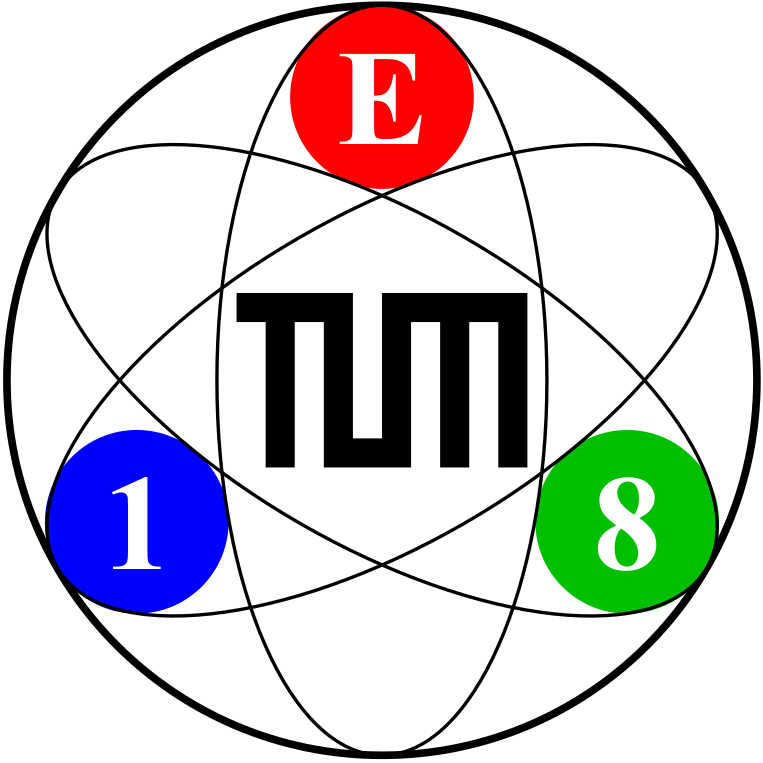
\includegraphics[width=0.8\textwidth]{E18Logo.png}
    \caption{Results of the threshold scan for Citiroc1A of FPGA 1 and FPGA 2.}
    \label{fig:threshold_scan}
\end{figure}
The differantiated data of the threshold scan is shown in Figure \ref{fig:threshold_scan_diff}.


\section{S-curve analysis}
In order to determine the optimal threshold and caracterize the noise of the Citiroc1A ASICs of FPGA 1 and FPGA 2, an S-curve analysis was performed.
\newline
The falling edge of the pedestal was fitted with the S-curve described in Section \ref{sec:noise_theory}
\newline
The results of the S-curve analysis are shown in Figure \ref{fig:S_curve}.
\begin{figure}[H]
    \centering
    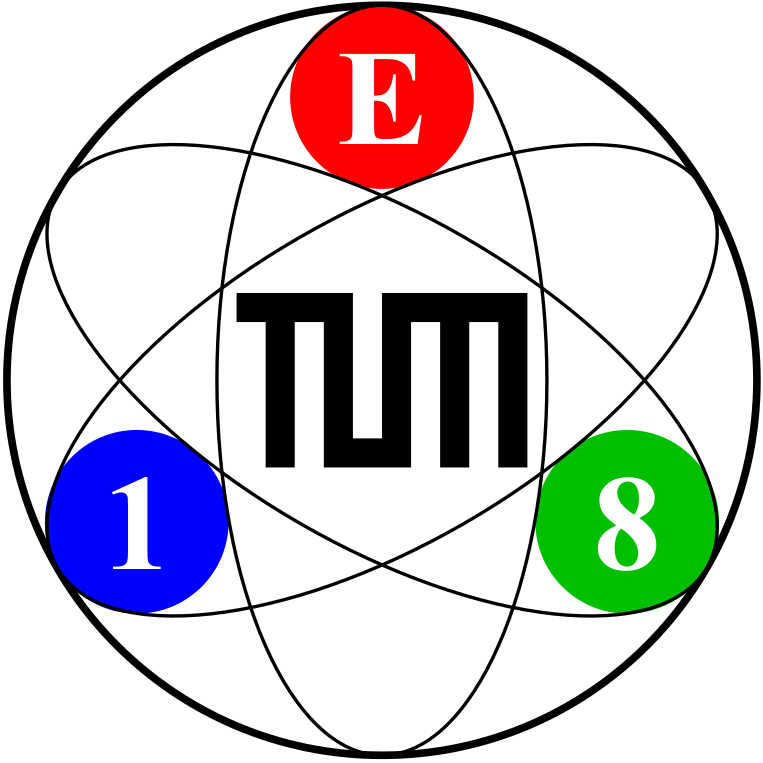
\includegraphics[width=0.8\textwidth]{E18Logo.png}
    \caption{Results of the S-curve analysis for Citiroc1A of FPGA 1 and FPGA 2.}
    \label{fig:S_curve}
\end{figure}
The mean $\mu$ and the standard deviation $\sigma$ of the noise distribution that were determined from the S-curve fits and are shown in Appendix \ref{}.



